\documentclass[12pt,a4paper]{article}

\usepackage[margin=2.5cm]{geometry}
\usepackage{graphicx}
\usepackage{booktabs}
\usepackage{array}
\usepackage{parskip}

\title{Superstore Sales Analysis\\Business Recommendation Report}
\author{}
\date{}

\begin{document}
\maketitle

\section*{Executive Summary}

This report analyses Superstore sales data across four US regions to identify
profit inefficiencies and provide actionable business recommendations.

The Central region achieves only 7.92\% profit margin --- nearly half of the West
region's 14.94\%. Statistical analysis across 45 states confirms that high discount
rates are strongly associated with low margins ($r = -0.905$, $p < 0.0001$).
Further investigation reveals that the losses originate from two distinct problems:
a Central-specific discount policy failure (Appliances, Furnishings, Binders),
and a company-wide structural pricing issue (Tables, Machines, Bookcases).

\section*{Key Findings}

\subsection*{Finding 1 --- Central has the lowest profit margin}

Central region generates \$501K in sales but achieves only 7.92\% profit margin
--- nearly half of West's 14.94\%, despite having higher sales than South.

\begin{figure}[htbp]
  \centering
  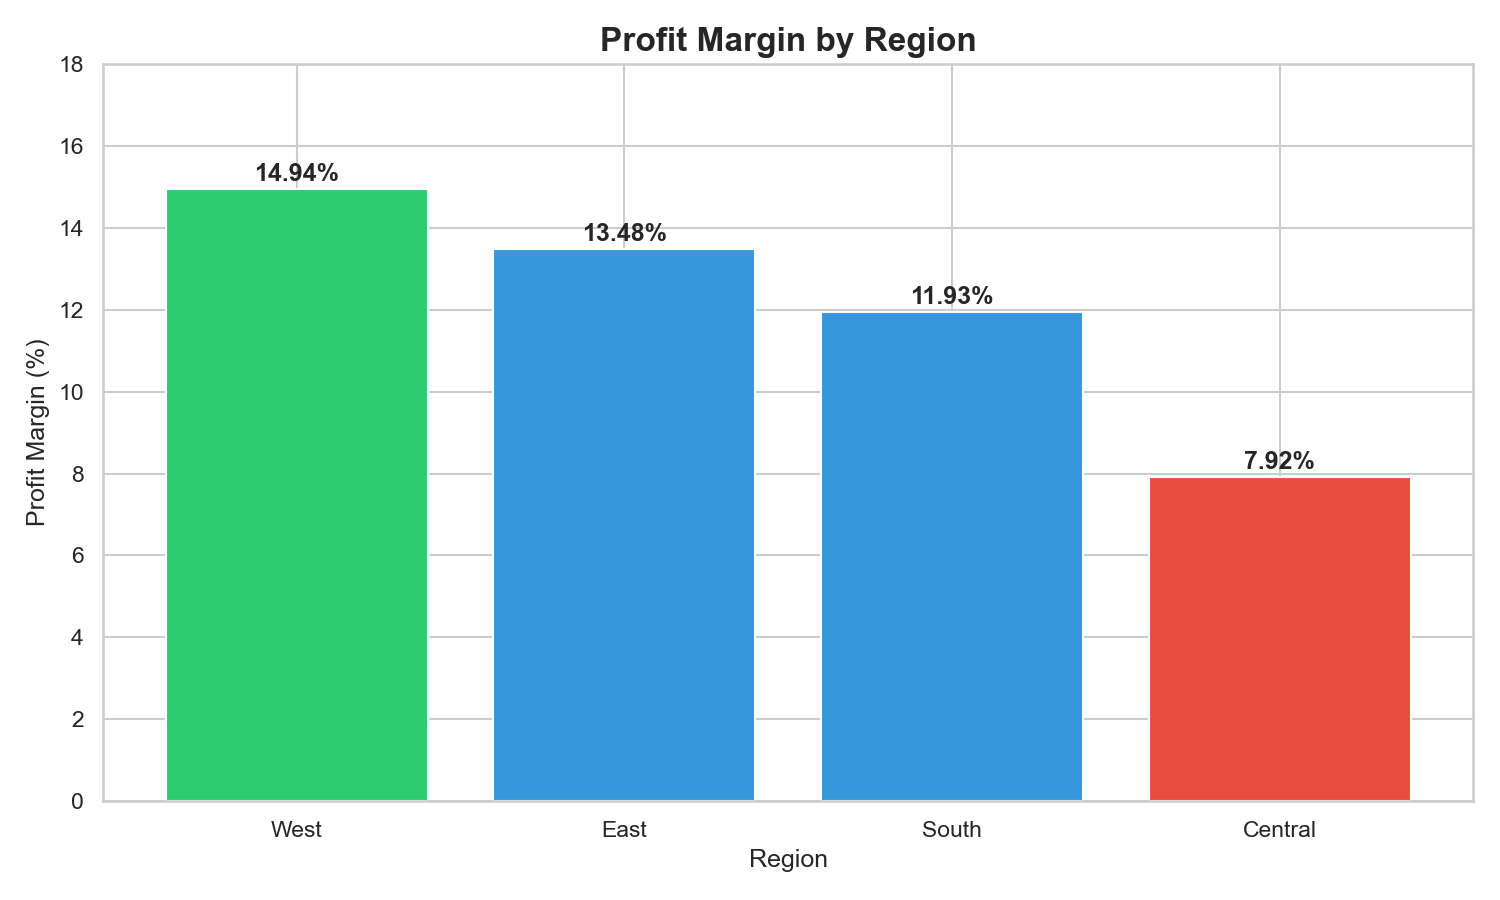
\includegraphics[width=0.85\textwidth]{chart1_region_margin.png}
\end{figure}

\subsection*{Finding 2 --- Central over-discounts compared to other regions}

Central's average discount of 24\% is more than double West's 11\%.
Empirical analysis shows that orders discounted above 20\% begin to generate
negative average profit --- establishing 20\% as the data-driven breakeven threshold.
27.7\% of Central's orders exceed this threshold, compared to 5.3\% in West.

\begin{figure}[htbp]
  \centering
  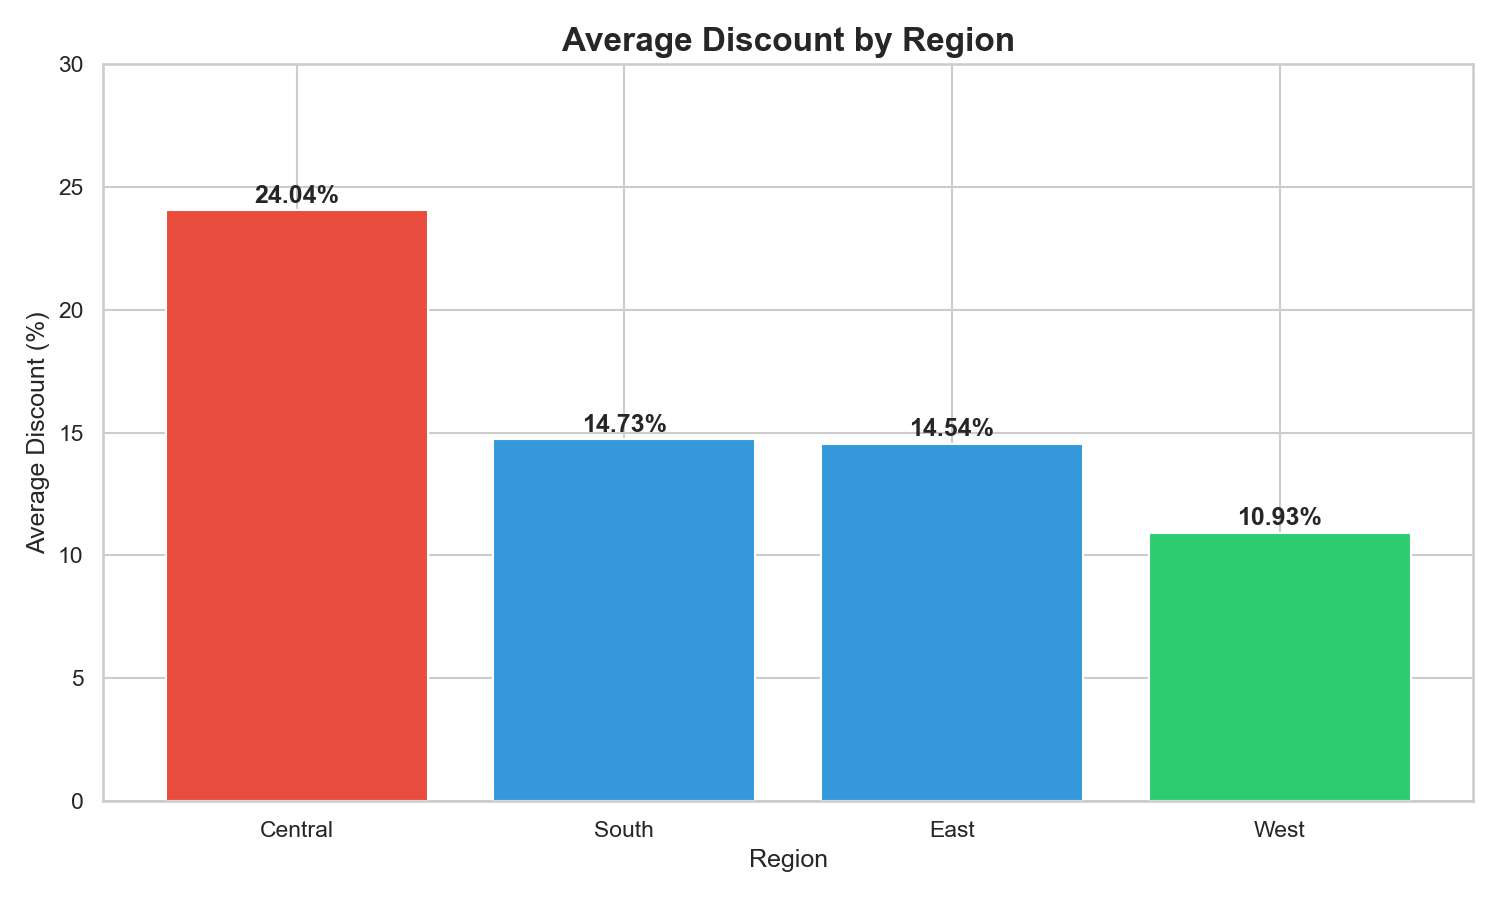
\includegraphics[width=0.85\textwidth]{chart2_region_discount.png}
\end{figure}

\subsection*{Finding 3 --- 7 sub-categories are losing money in Central}

7 out of 17 sub-categories in Central generate negative profit, accounting for
a combined loss of \$15,294. Furnishings alone loses \$3,906 despite \$15,254 in
sales. All seven loss-making sub-categories carry average discounts above
the 20\% breakeven threshold.

\begin{figure}[htbp]
  \centering
  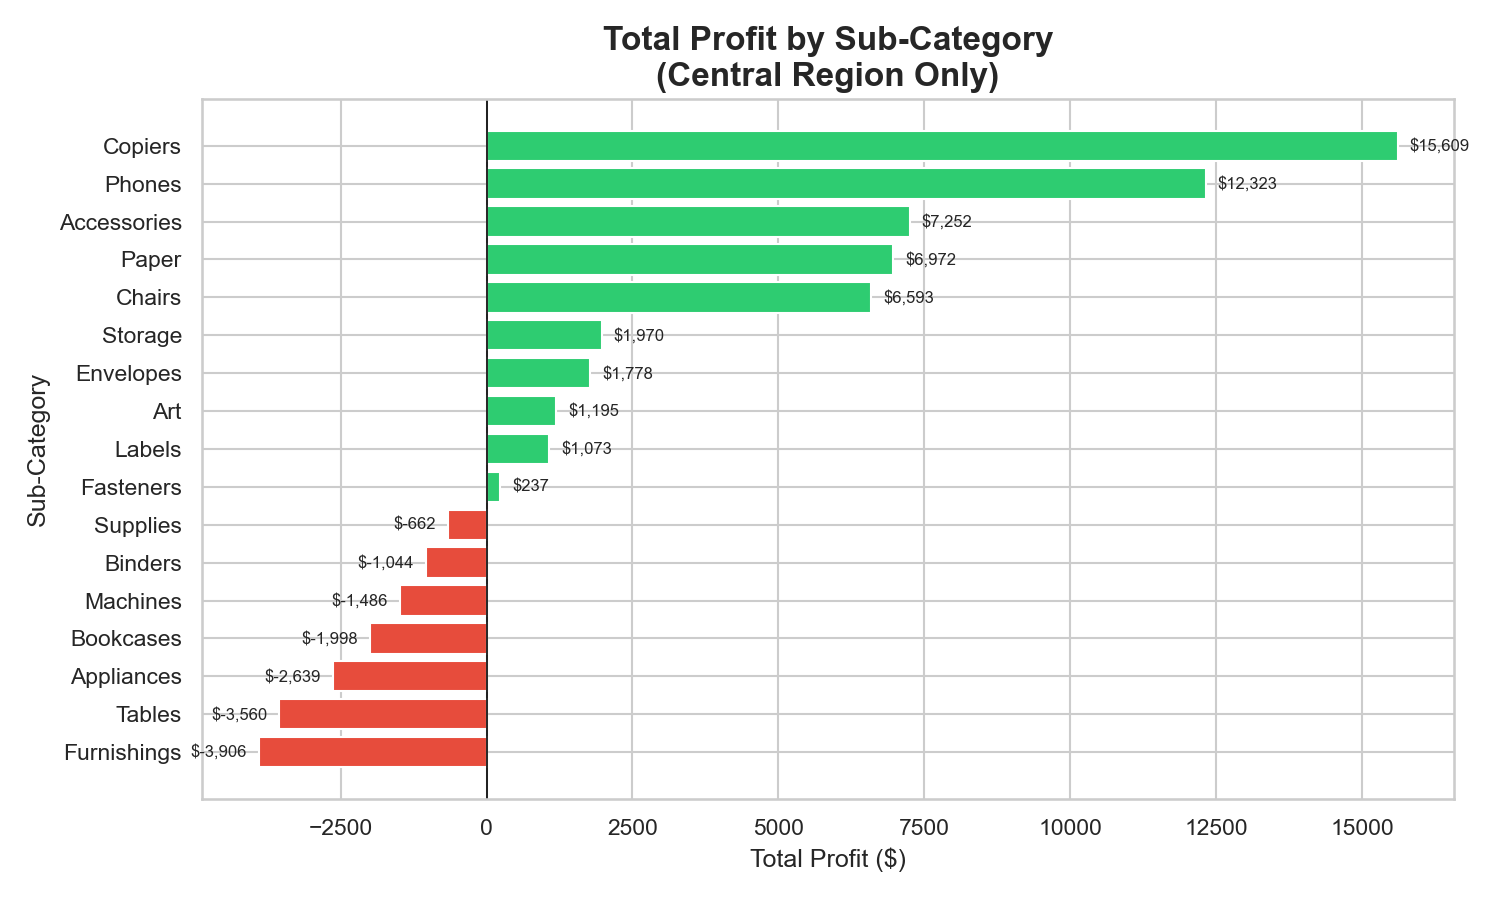
\includegraphics[width=0.85\textwidth]{chart3_central_subcategory.png}
\end{figure}

\subsection*{Finding 4 --- Orders above the 20\% breakeven are almost universally unprofitable}

The scatter plot confirms that once the discount rate crosses 20\%, profit
collapses across all three product categories. The 20\% threshold is not an
arbitrary choice --- it was derived empirically from the data in Finding 2.

\begin{figure}[htbp]
  \centering
  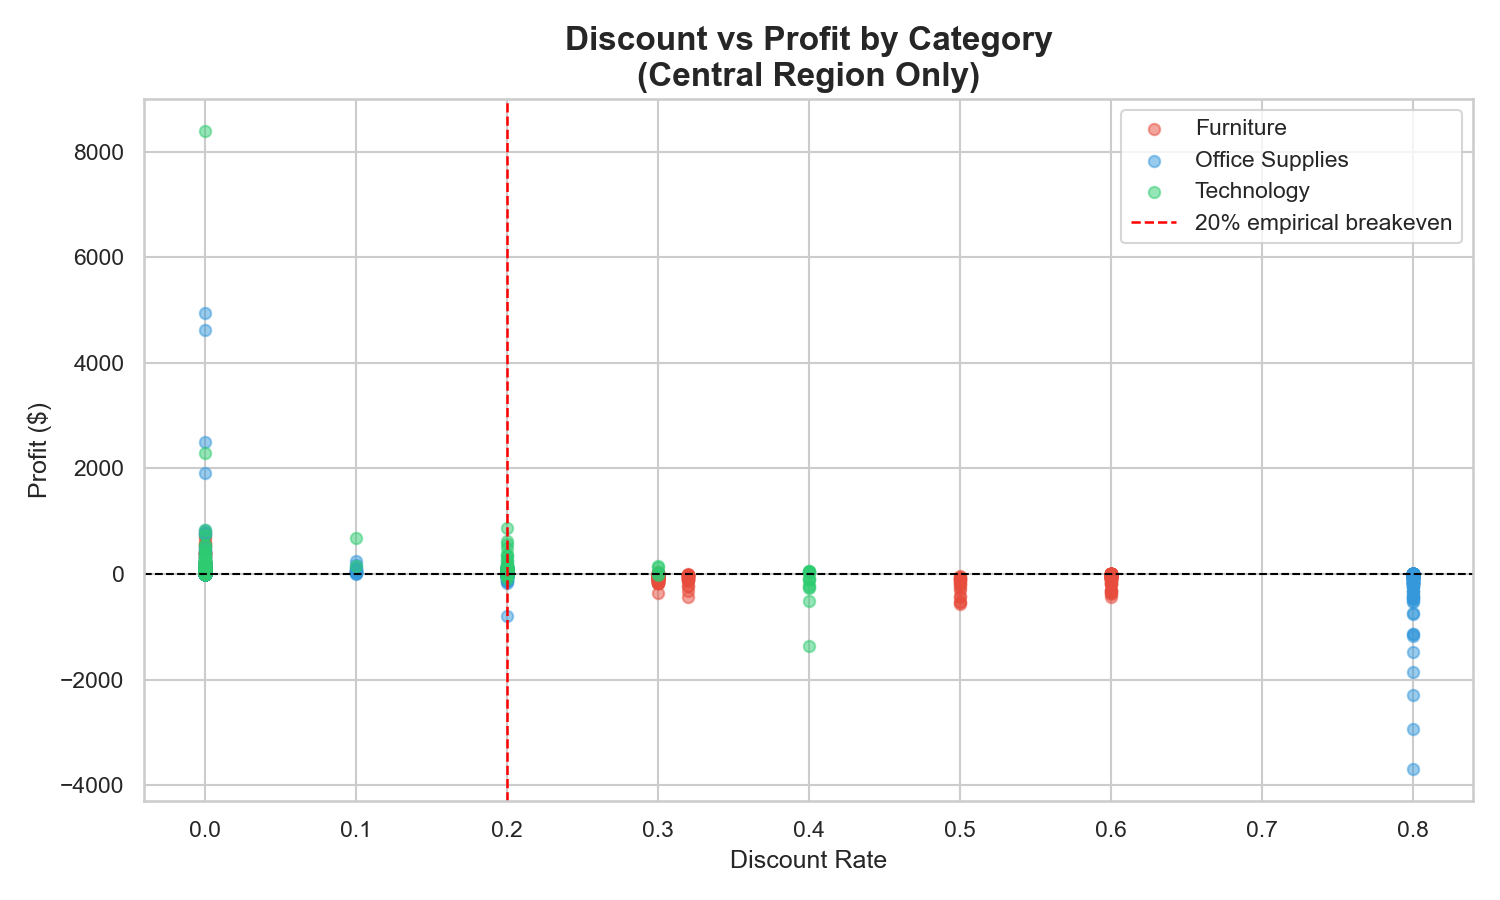
\includegraphics[width=0.85\textwidth]{chart4_discount_vs_profit.png}
\end{figure}

\subsection*{Finding 5 --- Discounting is a statistically validated driver of margin erosion}

To move beyond a regional observation, the analysis was extended to 45 US states.
The Pearson correlation between each state's high-discount order rate and its profit
margin is $r = -0.905$ ($p < 0.0001$, $n = 45$) --- a very strong, statistically
significant negative relationship. To rule out product mix as a confounding variable,
the correlation was repeated within each product category separately:
Furniture ($r = -0.757$), Office Supplies ($r = -0.919$), and Technology ($r = -0.669$)
all show the same pattern independently. This rules out the alternative explanation
that Central simply sells more inherently low-margin products.

\begin{figure}[htbp]
  \centering
  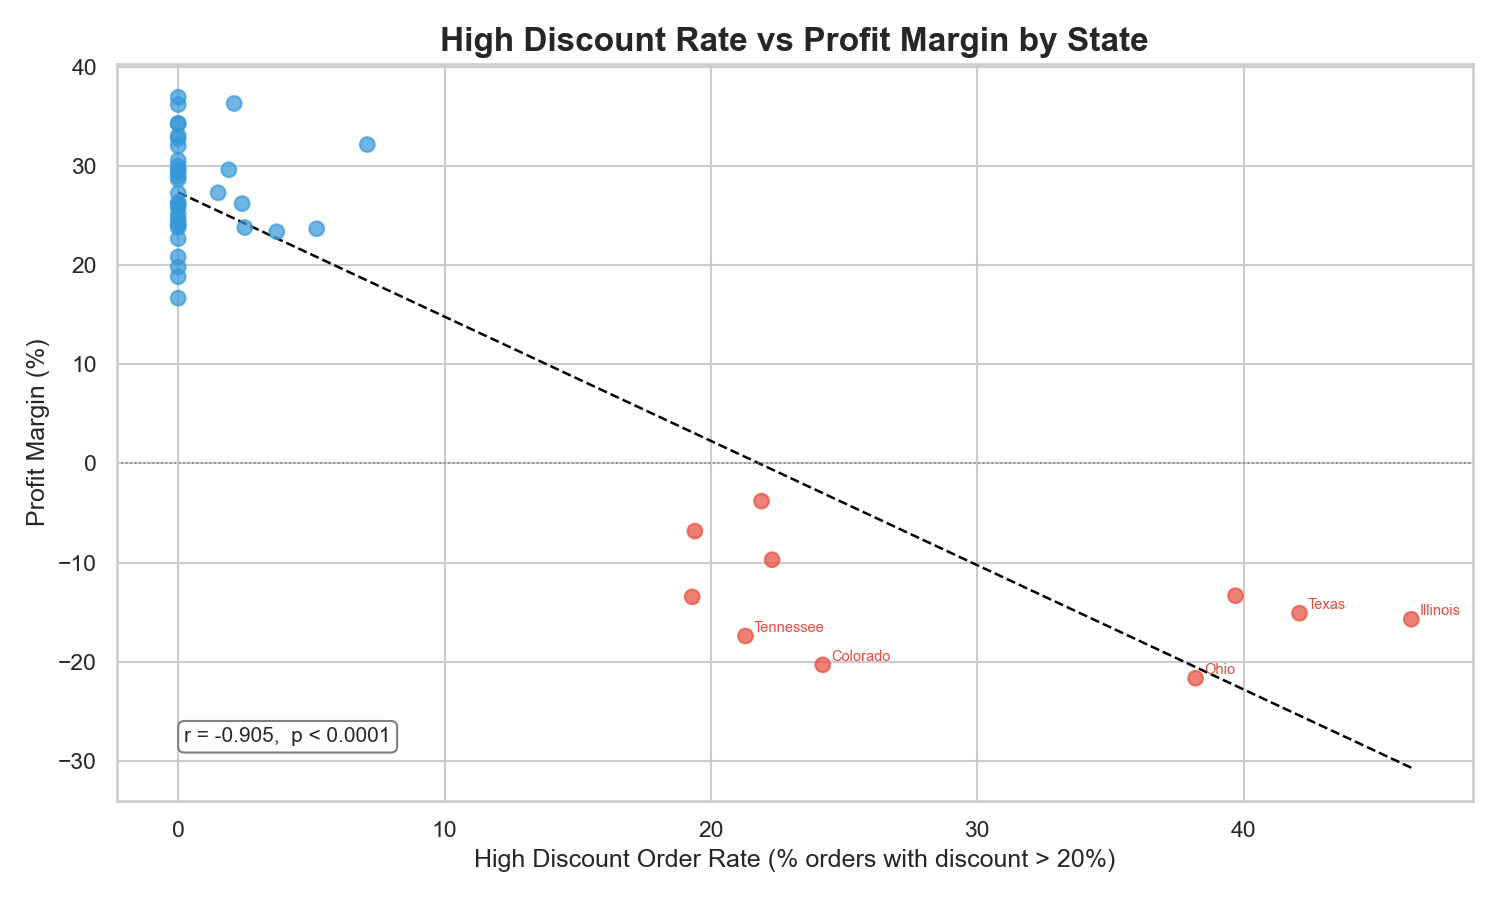
\includegraphics[width=0.85\textwidth]{chart5_state_discount_vs_margin.png}
\end{figure}

\subsection*{Finding 6 --- Two distinct problems require two different solutions}

Cross-region comparison of the 7 loss-making sub-categories reveals two groups:

\textbf{Group A --- Central-specific over-discounting:}
Appliances (Central 44.9\% vs other regions avg 7.2\%),
Furnishings (40.4\% vs 7.3\%), and Binders (50.9\% vs 33.7\%).
Other regions sell these same products profitably at low discount.
This is a Central regional management problem.

\textbf{Group B --- Company-wide structural issue:}
Tables (Central 26.2\% vs others 26.6\%), Machines (+2.2\%), and Bookcases (+5.0\%).
All four regions discount these products at similar levels.
Reducing Central's discount alone would not resolve these losses.
The issue lies in the product cost structure or list pricing across the business.

\begin{figure}[htbp]
  \centering
  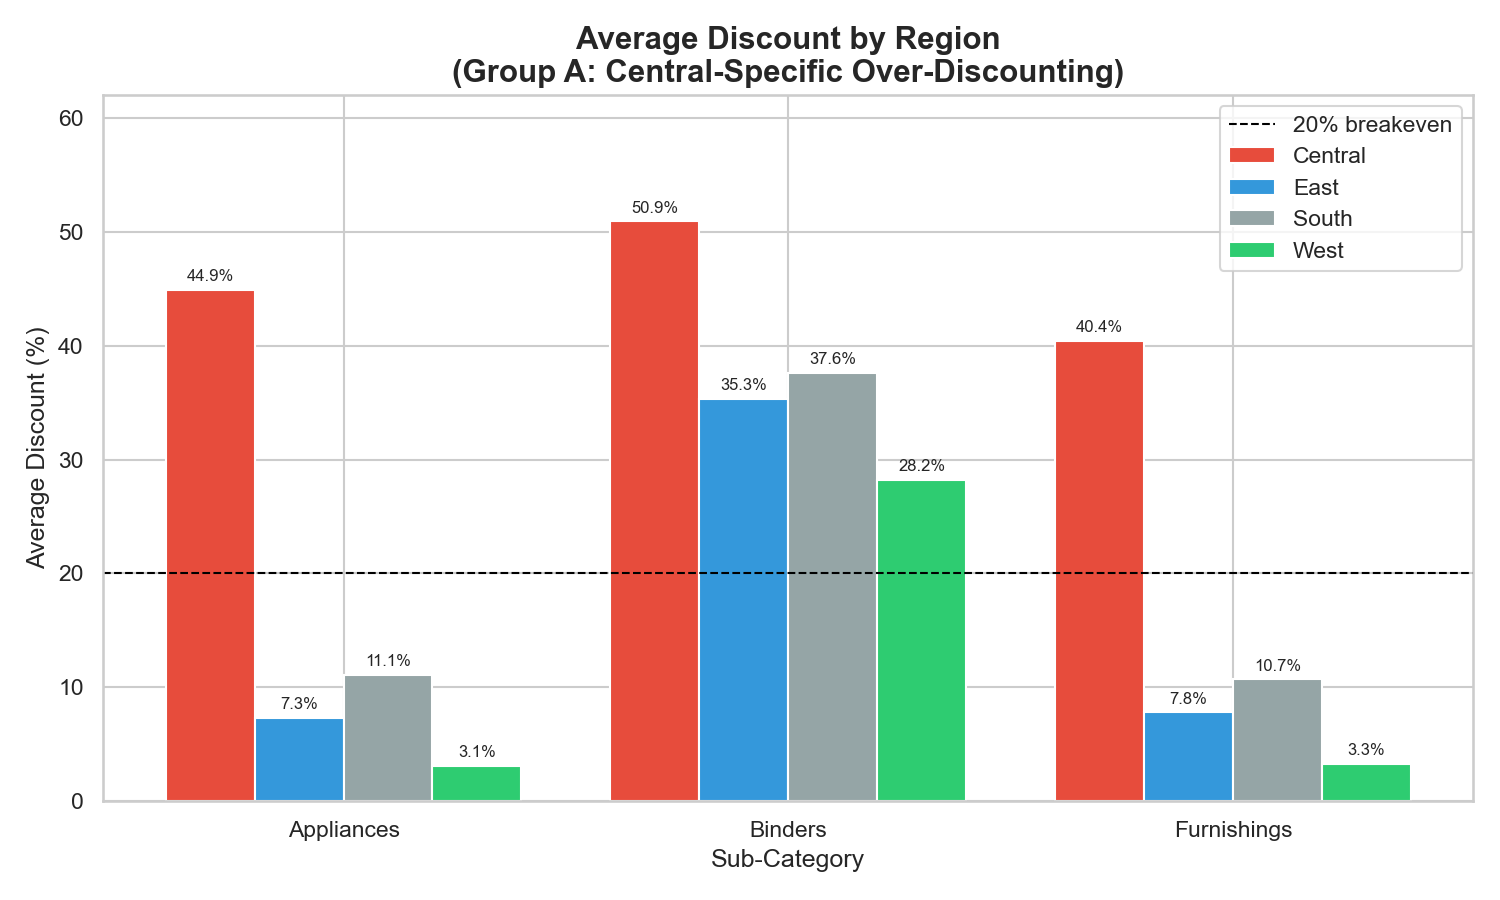
\includegraphics[width=0.85\textwidth]{chart6_group_a_discount_by_region.png}
\end{figure}

\section*{Business Recommendations}

\subsection*{For Central Regional Management}

\begin{tabular}{>{\raggedright\arraybackslash}p{0.5cm}>{\raggedright\arraybackslash}p{8cm}>{\raggedright\arraybackslash}p{4.5cm}}
  \toprule
  \textbf{\#} & \textbf{Recommendation} & \textbf{Expected Impact} \\
  \midrule
  1 &
  Cap discount authorisation at 20\% for Appliances and Furnishings.
  Other regions sell these products profitably at under 10\% discount. &
  Eliminate \$6,545 combined loss from Appliances and Furnishings \\
  \addlinespace
  2 &
  Review Binders discount policy. Central discounts at 50.9\% vs 33.7\%
  in other regions. Align with company average to reduce losses. &
  Recover portion of \$1,044 current loss \\
  \addlinespace
  3 &
  Pilot a discount cap of 20\% across all high-discount sub-categories
  for one quarter and track margin outcomes to validate causal effect. &
  Empirically confirm the discount--margin relationship \\
  \bottomrule
\end{tabular}

\subsection*{For Company Leadership}

\begin{tabular}{>{\raggedright\arraybackslash}p{0.5cm}>{\raggedright\arraybackslash}p{8cm}>{\raggedright\arraybackslash}p{4.5cm}}
  \toprule
  \textbf{\#} & \textbf{Recommendation} & \textbf{Expected Impact} \\
  \midrule
  4 &
  Review cost structure and list pricing for Tables, Machines, and Bookcases.
  All regions lose money on these products at current discount levels. &
  Address \$9,045 structural loss across all regions \\
  \addlinespace
  5 &
  Evaluate whether the current discount programme for these product lines
  generates sufficient customer retention or volume uplift to justify the losses. &
  Evidence-based decision on whether to reprice or discontinue heavy discounting \\
  \bottomrule
\end{tabular}

\section*{Conclusion}

Central's 7.92\% profit margin is the result of two overlapping problems.
The first is a regional discount policy failure: Central's sales team grants
Appliances and Furnishings discounts 5--6$\times$ higher than any other region,
with no evident justification. The second is a company-wide structural issue:
Tables, Machines, and Bookcases are unprofitable at the discount levels
currently applied across all regions.

Addressing both requires different actions at different levels of the organisation.
Central management should immediately review and cap discount authorisation
for Group A sub-categories. Company leadership should commission a separate
review of Group B product line economics to determine whether current pricing
is sustainable.

\vspace{2em}
\noindent\small Analysis conducted using SQL (SQLite3), Python (Pandas, Matplotlib,
Seaborn, SciPy), \LaTeX

\end{document}
